\documentclass[a4paper, 11pt]{article} 





%%% PACKAGES
\usepackage{graphicx} 
\usepackage[parfill]{parskip} % Activate to begin paragraphs with an empty line rather than an indent
\usepackage{booktabs} % for much better looking tables
\usepackage{threeparttable} % three-part-table
\usepackage{array} % for better arrays (eg matrices) in maths
\usepackage{paralist} % very flexible & customisable lists (eg. enumerate/itemize, etc.)
\usepackage{verbatim} % adds environment for commenting out blocks of text & for better verbatim
\usepackage[utf8, latin1]{inputenc} 
\usepackage{subfig} % make it possible to include more than one captioned figure/table in a single float
\usepackage{floatrow} % add notes below figure
\usepackage{lscape} %turn landscape
\usepackage{multirow}
\usepackage{amsmath} %math formatting
\usepackage{amssymb} %math formatting
\usepackage{tabulary} %table formatting
\usepackage{xcolor} %text color for annotations
\usepackage[colorlinks, citecolor=blue]{hyperref} % makes for easy anchor tags in document

%formatting allows footnotes to keep black color
\makeatletter
\def\@footnotecolor{red}
\define@key{Hyp}{footnotecolor}{%
	\HyColor@HyperrefColor{#1}\@footnotecolor%
}
\def\@footnotemark{%
	\leavevmode
	\ifhmode\edef\@x@sf{\the\spacefactor}\nobreak\fi
	\stepcounter{Hfootnote}%
	\global\let\Hy@saved@currentHref\@currentHref
	\hyper@makecurrent{Hfootnote}%
	\global\let\Hy@footnote@currentHref\@currentHref
	\global\let\@currentHref\Hy@saved@currentHref
	\hyper@linkstart{footnote}{\Hy@footnote@currentHref}%
	\@makefnmark
	\hyper@linkend
	\ifhmode\spacefactor\@x@sf\fi
	\relax
}%
\makeatother
\hypersetup{footnotecolor=black}


\renewcommand{\thesection}{\Alph{section}.}

\title{EDLD 650: Data Analysis and Replication Exercise (DARE) 3}
\author{David D. Liebowitz}
\date{Due: Feb. 14, 2022} 

\begin{document}
\maketitle



\section{Baseline randomization checks (1 points)}



\begin{enumerate}
	\item[A1.] In \autoref{tab:descriptives}, we present evidence that the randomization process produced balanced baseline characteristics by family income, gender and initial level of reading fluency. Across all three measures, mean differences are both small in magnitude and statistically indistinguishable from zero. Further, an omnibus $F$-test produces a $p$-value of 0.820, and we fail to reject the null hypothesis that there are no differences on these variables jointly across the treated and untreated individuals. Even if we were to have detected statistical differences in these baseline characteristics, it would not invalidate the causal claims of the study as the two groups (treatment and control) were randomized to their conditions, and thus are equal in expectation in the population. Such differences might arise from sampling idiosyncrasy and could be addressed post hoc through the inclusion of these covariates in our main analysis.
\end{enumerate}

\begin{table}
	
	\caption{Descriptive statistics by assigned EL status \label{tab:descriptives}}
\centering
\begin{tabular}[t]{lcccc}
	\toprule
	
& Not EL $(N=945)$ & EL $(N=1221)$ & Total $(N=2166)$ & $p$-value \\
\midrule
\textbf{Language Score} & & & & \textless{} 0.001 \\
~~~Mean (SD) & 17.62 (3.32) & 14.55 (4.89) & 15.89 (4.54) & \\
\textbf{Reading Score} & & & & \textless{} 0.001 \\
~~~Mean (SD) & 13.41 (4.57) & 10.79 (4.72) & 11.94 (4.83) & \\
\textbf{K Literacy Score} & & & & \textless{} 0.001 \\
~~~Mean (SD) & -0.49 (0.96) & -1.03 (0.80) & -0.80 (0.91) & \\
\textbf{K Math Score} & & & & \textless{} 0.001 \\
~~~Mean (SD) & -0.50 (1.00) & -1.07 (1.00) & -0.82 (1.04) & \\
\textbf{SES} & & & & \textless{} 0.001 \\
~~~Mean (SD) & -0.21 (0.91) & -0.69 (0.68) & -0.48 (0.82) & \\
\textbf{Female} & & & & 0.396 \\
~~~Mean (SD) & 0.51 (0.50) & 0.49 (0.50) & 0.50 (0.50) & \\
\textbf{Rural school} & & & & \textless{} 0.001 \\
~~~Mean (SD) & 0.14 (0.34) & 0.08 (0.27) & 0.11 (0.31) & \\
\textbf{Hispanic/Latinx} & & & & \textless{} 0.001 \\
~~~Mean (SD) & 0.50 (0.50) & 0.75 (0.44) & 0.64 (0.48) & \\
\bottomrule
\end{tabular}
\end{table}

\section{Replication and Extension 9 points)}


\begin{enumerate}
	\item[B1.] In \autoref{tab:ols}, we present estimates describing the relationship between post-intervention reading comprehension scores and students' rates of attendance in a seven-week after-school READ180 program. Model 1 estimates reading comprehension as a function of program participation and baseline reading score, Model 2 includes student background characteristics, and Model 3 adds school fixed effects. The estimated magnitude of the relationship across all three models suggests that full participation in a seven-week READ180 intervention increases reading comprehension scores by just less than 10 scale score points. However, these estimates should not be understood as assessing the causal effect of READ180 program attendance despite the fact that students were randomized into the program. While assignment to the program was random, students' rates of participation were not. Attendance rates ranged from 100 percent to less than 20 percent. These differences likely bias the estimates in Table 2 as students who attended READ180 at different rates are likely different in both observable and unobservable ways that are also related to their final test score outcomes.

	
% Table created by stargazer v.5.2.2 by Marek Hlavac, Harvard University. E-mail: hlavac at fas.harvard.edu
% Date and time: Mon, Feb 14, 2022 - 12:02:31 PM
\begin{table}[!htbp] \centering 
  \caption{Na{\"i}ve OLS estimates of the effects of READ180 attendance on reading comprehension score} 
  \label{tab:ols} 
\begin{tabular}{@{\extracolsep{5pt}}lccc} 
\\[-1.8ex]\hline \hline \\[-1.8ex] 
\\[-1.8ex] & (1) & (2) & (3)\\ 
\hline \\[-1.8ex] 
 Full READ180 Attend & 9.932$^{***}$ & 9.662$^{***}$ & 9.672$^{***}$ \\ 
  & (2.265) & (2.261) & (2.265) \\ 
\hline \\[-1.8ex] 
Student Chars & No & Yes & Yes \\ 
School Fixed Effects & No & No & Yes \\
\hline \\[-1.8ex]  
Observations & 312 & 312 & 312 \\ 
R$^{2}$ & 0.732 & 0.736 & 0.740 \\ 
\hline 
\hline \\[-1.8ex] 
\multicolumn{4}{l}{\emph{Notes:} *p$<$0.05, **p$<$0.01, ***p$<$0.001. Cells report coefficients} \\ 
\multicolumn{4}{l}{and associated standard errors} \\ 
\end{tabular} 
\end{table} 


	\item[B2.] In \autoref{fig:box}, we present the range, interquartile range and median value of final reading comprehension scores for students who were assigned to a traditional after-school program and for students assigned to the READ180 intervention. The mean performance level of students assigned to the READ180 intervention was 9.01 scale score points higher than those assigned to the district after-school program. With an associated $t$-statistic of 2.43, we can reject the null hypothesis that there is no difference, on average in the population, in the final performance of these two groups.

	\begin{figure} 
		\begin{center} 
			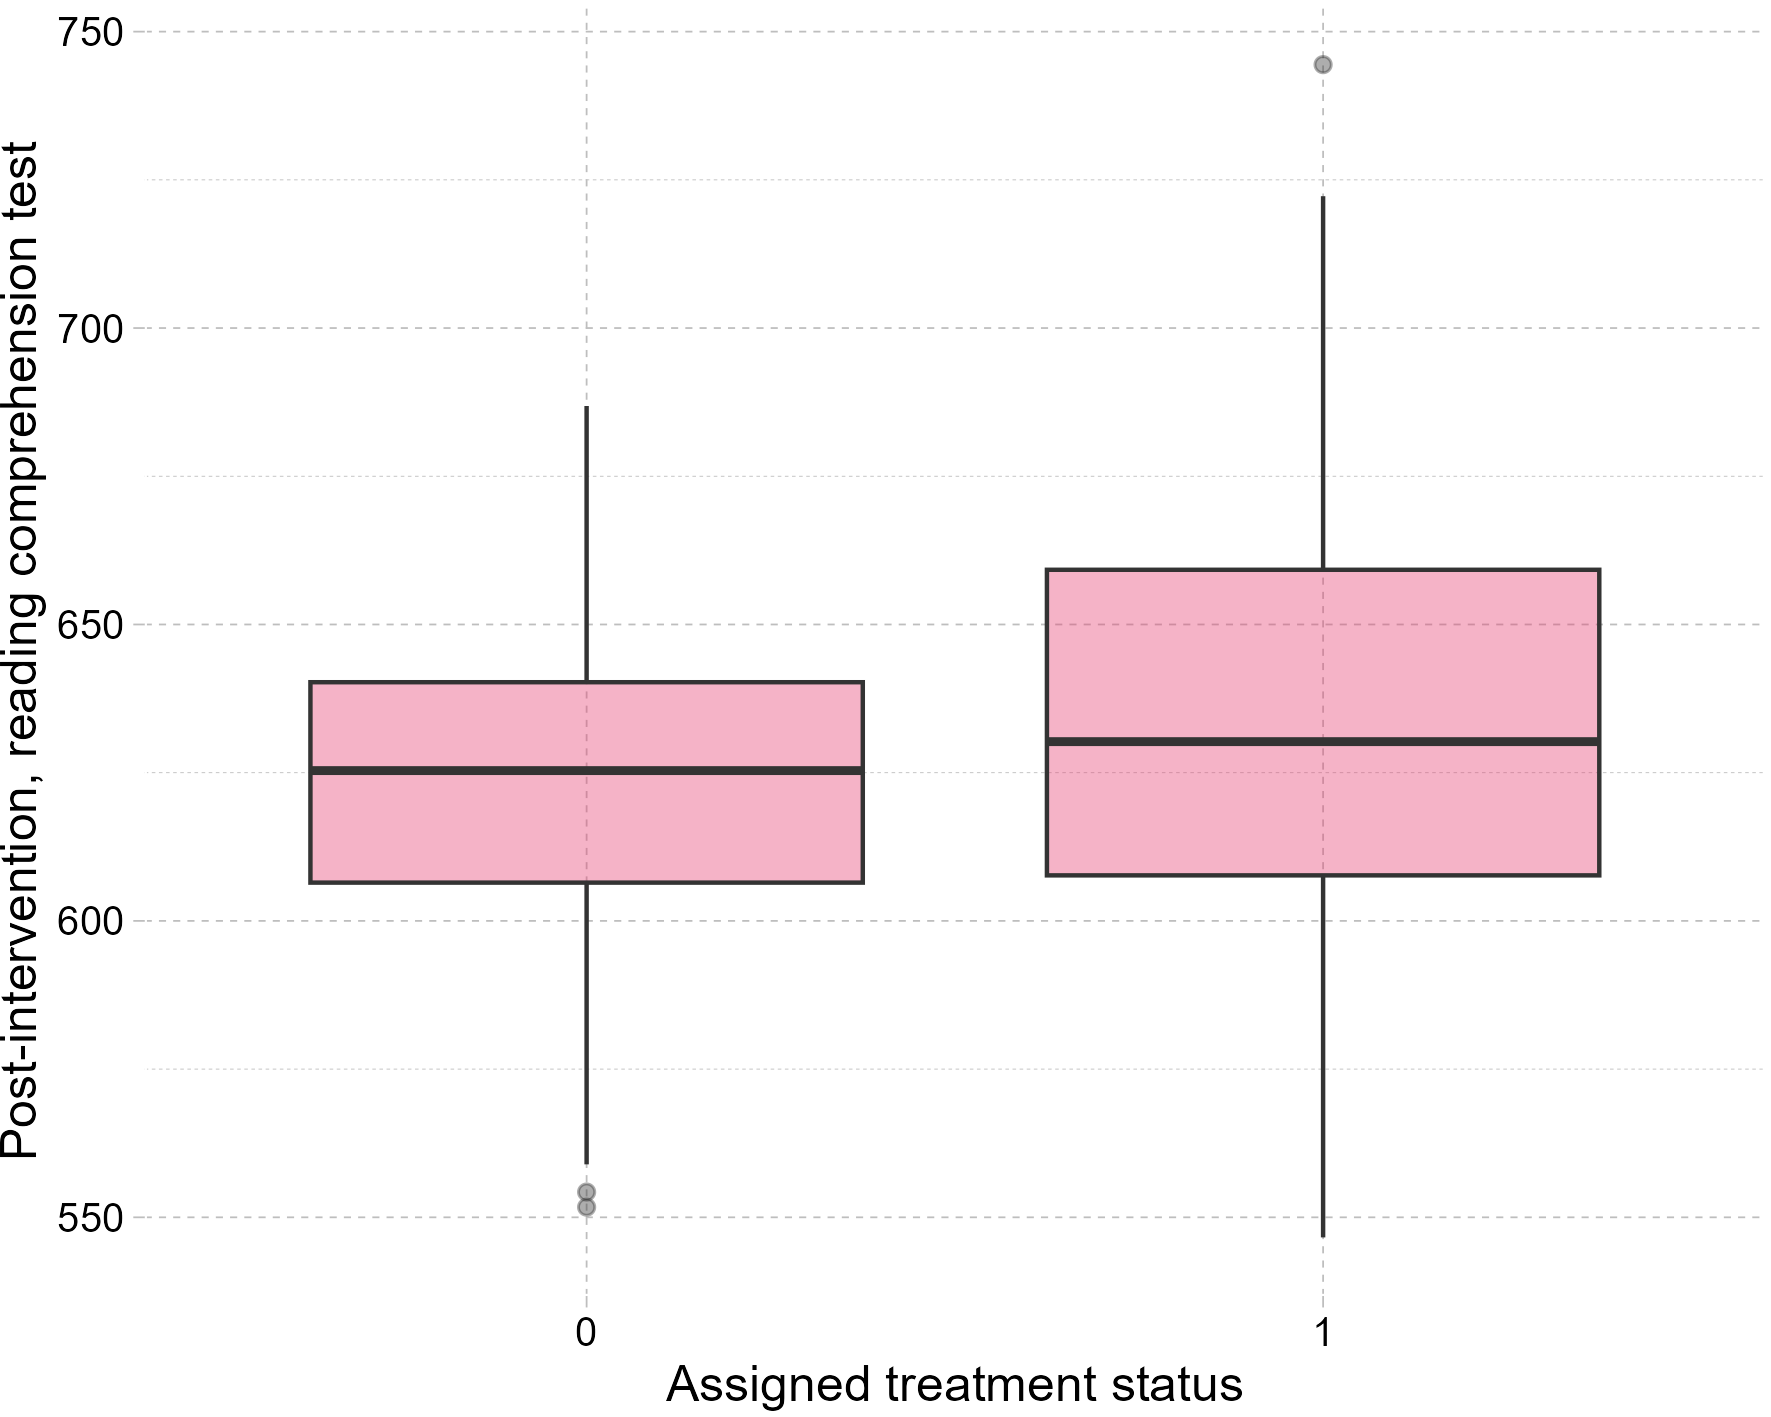
\includegraphics[scale=0.7]{figures/mean_out_compare.png}
			\caption{Post-intervention reading comprehension score, by assigned after-school program} \label{fig:box}
		\end{center}
	\end{figure}

	\item[B3.] In \autoref{tab:itt}, we present a taxonomy of intent-to-treat (ITT) estimates of the effect of being assigned to the READ180 intervention on a post-program reading comprehension test. Model 1 is a simple bivariate regression and mirrors the results from B2. The inclusion of starting reading fluency scores and student characteristics in Model 2 substantially improves the overall explanatory power of our model, and as a result shrinks the standard errors on our treatment indicator. It also attenuates the magnitude of the program effect by around 1 scale score point. Subsequent estimates incorporate school fixed effects (Models 3 and 4), and cluster standard errors at the school level (Model 5)\footnote{We include Models 3 and 4 for pedagogic purposes. They estimate the same model using different R packages and return identical results.}. All of the covariate adjusted estimates return stable coefficients on the effect of assignment into the READ180 program of a reading comprehension score boost of approximately 8 scale score points.

	\begin{table}

\caption{Intent-to-Treat estimates of random assignment to READ180 after-school intervention \label{tab:itt}}
\centering
\begin{threeparttable}
\begin{tabular}[t]{lccccc}
\hline 
\hline \\[-1.8ex] 
  & (1) & (2) & (3) & (4) & (5)\\
\midrule
Assigned to Read180 & 9.014* & 8.037*** & 8.003*** & 8.003*** & 8.003**\\
 & (3.703) & (1.935) & (1.935) & (1.935) & (0.762)\\
\midrule
Student Chars & No & Yes & Yes & Yes & Yes\\
School Fixed Effects & No & No & Yes & Yes & Yes\\
School-Clustered SEs & No & No & No & No & Yes\\
Num.Obs. & 312 & 312 & 312 & 312 & 312\\
R2 & 0.019 & 0.736 & 0.739 & 0.739 & 0.739\\
RMSE & 32.60 & 16.92 & 16.82 & 16.82 & 16.82\\
\hline 
\hline \\[-1.8ex] 
\end{tabular}
\begin{tablenotes}
\item \small \textit{Notes}: Cells report coefficients and associated standard errors.
\end{tablenotes}
\end{threeparttable}
\end{table}



	\item[B4.] We implement an instrumental variables approach in a two-stage least squares framework to estimate the effect of READ180 attendance on reading comprehension outcomes. Specifically, we rely on randomized assignment into the READ180 program as an instrument to estimate the effect of endogenous observed READ180 attendance on later comprehension test scores. Formally, we fit:
	\begin{equation}
	\text{READ180ATTEND}_i = \alpha_0 + \alpha_1 \text{TREAT}_i + \textbf{X}_i \theta + \delta_i
	\end{equation}
	\begin{equation}
	\text{READCOMP}_i = \beta_0 + \beta_1 \hat{READ180ATTEND}_i + \textbf{X}_i \theta + \epsilon_i
	\end{equation}
	where \textit{READ180ATTEND}$_{i}$ is scaled between 0 and 1 based on the proportion of days out of 84 that each individual student attended, \textit{TREAT} is defined as 1 for individuals assigned to the READ180 intervention and 0 otherwise, and \textbf{X}$_{i}$ is a vector of pre-assignment baseline characteristics. 
	
	Our approach relies on three key assumptions to defend its causal interpretation. First, our instrument (assignment to READ180) should predict rates of attendance in READ180. As expected, given the random assignment we leverage, our instrument is strongly predictive of daily attendance in READ180, with an associated $t$-statistic of over 40. Our overall first-stage model has an $F$-statistic just shy of 1,670, well exceeding conventional thresholds. Second, our instrument should be exogenous, that is uncorrelated with our first-stage residuals. We note that the randomized assignment to the READ180 condition should preclude any unobserved differences in READ180 attendance rates across treatment and control. Further, our results in Table 1 indicate that (on the observables), randomization appears to have been well executed. Thus, we take this as strong evidence that our second assumption has been met. Finally, our instrument should affect our final outcome, post-intervention reading comprehension test scores, through no other pathway than through students' attendance in READ180. Logically, this assumption should be satisfied in this randomized setting.
	
	In \autoref{tab:tot}, we present results from a series of instrumental variables estimates of the effect of attendance in a READ180 after-school intervention on reading comprehension. Model 1 is the unconditional model. We interpret it as full attendance of 84 days in an after-school READ180 intervention increases reading comprehension scores by 11.5 scale points. The inclusion of student characteristics (Model 2) attenuates our main effect to 10.2 points but dramatically increases the explanatory power of our model and the precision of our primary estimate. The estimate in Model 2 is stable in magnitude and statistically robust to the inclusion of school fixed effects and the associated clustered standard errors (Models 3 and 4).\footnote{Intriguingly, our standard errors become smaller when we cluster them at the school level. This is due to the simulated data generating process. In these toy data, I randomly assigned students to schools and so schools explain none of the variation in test outcome. Further, recall that clustered standard errors asymptotically approach the true estimates as the number of clusters approaches and exceeds 50. Here, with only four clusters the clustered standard errors are biased \textit{downwards}. An important reminder that just because we can cluster standard errors does not mean we should.}

	\begin{table}

\caption{Treatment-on-the-Treated estimates of full participation in a seven-month READ180 after-school intervention \label{tab:tot}}
\centering
\begin{threeparttable}
\begin{tabular}[t]{lcccc}
\hline 
\hline \\[-1.8ex] 
  & (1) & (2) & (3) & (4)\\
\midrule
Predicted Read180 Attendance & 11.472* & 10.236*** & 10.208*** & 10.208***\\
 & (4.708) & (2.460) & (2.464) & (0.788)\\
\midrule
Student Chars & No & Yes & Yes & Yes\\
School Fixed Effects & No & No & Yes & Yes\\
School-Clustered SEs & No & No & No & Yes\\
Num.Obs. & 312 & 312 & 312 & 312\\
R2 & 0.021 & 0.736 & 0.740 & 0.740\\
RMSE & 32.57 & 16.90 & 16.79 & 16.79\\
\hline 
\hline \\[-1.8ex] 
\end{tabular}
\begin{tablenotes}
\item \small \textit{Notes}: Cells report coefficients and associated standard errors.
\end{tablenotes}
\end{threeparttable}
\end{table}


	\item[B5.] Our results indicate that late-elementary school students assigned to a seven-week after-school mixed-method literacy program improved their reading comprehension skills. Students randomly assigned to the READ180 Enterprise program improved reading comprehension scores by around 8 scale score points. We further estimate the causal effect of full program attendance for 84 days at around 10 scale score points. These correspond to effects of between one-quarter and one-third of a standard deviation (\textit{SD}), and we confidently rule out effects smaller than 0.15 \textit{SDs}. These represent substantial gains. Although not all students will fully participate, we note that even the offer of the program produces robust reading comprehension gains. These results should be understood in the context of the targeted population: low-performing students in four Massachusetts elementary schools. Further replication will be critical to confidently generalize these results to other student populations. 

\end{enumerate}


\end{document} 